\documentclass[11pt]{article}

\usepackage[a4paper,margin=1in]{geometry}
\usepackage{amsmath}
\usepackage{booktabs}
\usepackage{array}
\usepackage{graphicx}
\usepackage{float}
\usepackage{longtable}
\usepackage{listings}
\usepackage{caption}
\usepackage{subcaption}
\usepackage{xcolor}
\usepackage{parskip}
\usepackage{fancyhdr}
\usepackage[hidelinks]{hyperref}

\pagestyle{fancy}
\fancyhf{}
\fancyhead[L]{Spelling Corrector}
\fancyhead[R]{NLP Group Assignment -- Question 3}
\fancyfoot[C]{\thepage}
\renewcommand{\headrulewidth}{0.4pt}

\definecolor{codebg}{rgb}{0.95,0.95,0.95}
\lstset{
  backgroundcolor=\color{codebg},
  basicstyle=\ttfamily\small,
  breaklines=true,
  frame=single,
  numbers=left,
  numberstyle=\tiny,
  columns=fullflexible,
  keepspaces=true,
  showstringspaces=false
}

\title{\textbf{Building, Benchmarking, and Deploying\\ an Efficient Spelling Corrector}\\[0.5em]
\large NLP Group Assignment --- Question 3}

\author{\begin{minipage}{0.85\textwidth}\centering\textbf{Group 21:} Krishna Jhanwar (12341250), Siddharth Rai (12342050), Slok Tulsyan (12342080), Vasu Garg (12342330), Gaurav Kumar (12340790)\end{minipage}}

\date{September 8, 2026}

\begin{document}

\maketitle

\begin{abstract}
This report documents the design, implementation, and evaluation of a spelling corrector built on the NLTK Brown corpus, capable of correcting both \textit{non-word} errors (out-of-vocabulary misspellings) and \textit{real-word} errors (contextually incorrect but valid words) within an edit distance of one. Two independent candidate-generation strategies are implemented and compared: a brute-force edit-distance-1 generator, and the Symmetric Delete Spelling Correction (SymSpell) algorithm. The two are benchmarked head-to-head on a fixed batch of 1,000 misspelled words, showing a $\sim$5.8$\times$ speed-up for the Symmetric Delete method. The corrector is evaluated for accuracy on an automatically generated, edit-distance-1 test set drawn from 10\% of the Brown corpus sentences, and finally deployed as a live, interactive terminal application.
\end{abstract}

\section{Introduction}

Spelling correction is one of the oldest and most practically important problems in natural language processing. A useful corrector must handle two qualitatively different kinds of mistakes:

\begin{itemize}
\item \textbf{Non-word errors} --- the misspelled string is not a valid word at all (e.g. \textit{``sentnce''}), so any out-of-vocabulary token is immediately flagged and the job is to rank the plausible corrections.
\item \textbf{Real-word errors} --- the misspelled string happens to collide with another valid word (e.g. \textit{``sea''} instead of \textit{``see''}), so the word cannot be flagged from vocabulary membership alone; only the surrounding context reveals the mistake.
\end{itemize}

This assignment asks us to build both capabilities on top of the NLTK \textbf{Brown corpus}, compare two ways of generating single-edit candidate corrections, benchmark them for speed, and package the result as a live CLI tool. Section~2 covers corpus and model preparation, Sections~3 and~4 cover candidate generation and correction logic, Section~5 covers evaluation and the ``Speed Demon'' benchmark, Section~6 covers the interactive application, and Section~7 discusses results, limitations, and possible extensions. Full source code is reproduced in the Appendix.

\subsection{System overview}

Figure~\ref{fig:pipeline} sketches the overall data flow: the Brown corpus is processed once into a vocabulary, a unigram frequency table, and a bigram language model; these are shared by both candidate-generation methods and by the correction logic that sits on top of them; the same corrector object then powers both the offline evaluation harness and the live CLI.

\begin{figure}[H]
\centering
\begin{tabular}{|p{0.42\textwidth}|p{0.42\textwidth}|}
\hline
\multicolumn{2}{|c|}{\textbf{Brown Corpus} $\rightarrow$ \textbf{Vocabulary + Unigram Freq.}} \\
\multicolumn{2}{|c|}{\textbf{Bigram Model (Part 1)}} \\
\hline
\multicolumn{2}{|c|}{$\downarrow$} \\
\hline
\textbf{Method A}: Edit-Distance-1 & \textbf{Method B}: Symmetric Delete \\
(brute force, Part 2) & (pre-processed dict, Part 2) \\
\hline
\multicolumn{2}{|c|}{\textbf{Correction Logic (Part 3)}} \\
\multicolumn{2}{|c|}{Non-word: max frequency} \\
\multicolumn{2}{|c|}{Real-word: max bigram prob.} \\
\hline
\textbf{Evaluation \& Speed Demon} & \textbf{Live Terminal CLI} \\
(Part 4) & (Part 5) \\
\hline
\end{tabular}
\caption{End-to-end pipeline of the spelling corrector.}
\label{fig:pipeline}
\end{figure}

\section{Part 1: Corpus and Model Preparation}

\subsection{Vocabulary and unigram frequencies}

The Brown corpus is loaded via \texttt{nltk.corpus.brown.sents()}. Each sentence is lower-cased and filtered to purely alphabetic tokens, since numbers and punctuation have no meaningful ``edit distance 1'' correction. Word counts are accumulated with a \texttt{collections.Counter}:

\[
\mathrm{freq}(w) = \#\{\text{occurrences of } w \text{ in the corpus}\}, \qquad V = \{w : \mathrm{freq}(w) > 0\}
\]

\subsection{Bigram language model}

A bigram model estimates $P(w_2 \mid w_1)$ from corpus counts, with sentence boundaries marked by pseudo-tokens \texttt{<s>} and \texttt{</s>} so that sentence-initial and sentence-final words are also modeled. Raw maximum likelihood estimates,

\[
P_{\mathrm{MLE}}(w_2 \mid w_1) = \frac{C(w_1, w_2)}{C(w_1)},
\]

assign zero probability to any bigram never seen in training, which is fatal when comparing candidate phrases that are individually rare. We therefore use \textbf{add-one (Laplace) smoothing}:

\[
P(w_2 \mid w_1) = \frac{C(w_1, w_2) + 1}{C(w_1) + |V|}
\]

where $|V|$ is the vocabulary size (plus the two pseudo-tokens). Phrase probabilities are computed in \textbf{log-space} to avoid numerical underflow and to make comparisons between candidate phrases a simple subtraction:

\[
\log P(w_1 \ldots w_n) = \sum_{i=1}^{n} \log P(w_i \mid w_{i-1})
\]

\subsection{Caching}

Because building these tables from 56K+ sentences is the most expensive one-time step, the vocabulary, frequency table, bigram counts, and sentence list are pickled to \texttt{data/*.pkl} after the first run, so all later runs (evaluation, demo, CLI) load instantly instead of rebuilding.

\section{Part 2: Candidate Generation Methods}

Both methods below are meant to answer the same question --- \textit{``which vocabulary words are within one edit of this string?''} --- but they arrive at the answer through very different computational routes, which is exactly what the Speed Demon benchmark in Section~5 is designed to expose.

\subsection{Method A: Standard Edit-Distance-1 Generation}

Method A is the classical brute-force generator (in the style popularised by Norvig's spelling corrector). For a word of length $n$ it enumerates every string reachable by a single \textit{delete}, \textit{transpose}, \textit{replace}, or \textit{insert} operation:

\[
\begin{aligned}
\text{deletes} &: L + R[1:] \text{ for each split } (L, R) \\
\text{transposes} &: L + R[1] + R[0] + R[2:] \text{ for each split with } |R| > 1 \\
\text{replaces} &: L + c + R[1:] \text{ for each split, each letter } c \\
\text{inserts} &: L + c + R \text{ for each split, each letter } c
\end{aligned}
\]

This produces on the order of $26n + 25$ candidate strings, most of which are not real words; the raw set is intersected with the vocabulary to keep only valid candidates.

\textbf{Complexity:} $O(26n)$ string constructions per query word, each followed by an $O(1)$ average-case hash-set membership check --- i.e. $O(n)$ work scaled by the alphabet size.

\subsection{Method B: Symmetric Delete Spelling Correction}

Symmetric Delete (SymSpell) trades query-time work for a one-off pre-processing cost. \textbf{Pre-processing} (done once, offline): for every vocabulary word $w$, generate all of its single-character deletions and map each deletion string back to $w$ (plus an identity entry $w \mapsto w$):

\[
\text{delete\_dict}[d] \mathrel{+}= w \quad \text{for every } d \in \text{deletes}(w) \cup \{w\}
\]

\textbf{Query time}: for a misspelled word $q$, generate \textit{only} its own single-character deletions (plus itself) and look each one up directly in \texttt{delete\_dict} --- no alphabet loop at all:

\[
\text{candidates}(q) = \bigcup_{v \in \text{deletes}(q) \cup \{q\}} \text{delete\_dict}[v]
\]

Because deletion-based matching can, in rare cases, surface a pair of words whose \textit{true} edit distance is 2 (a known property of delete-delete matching), a cheap Levenshtein-distance-$\leq 1$ verification pass is applied to the (small) candidate set before it is returned, so Method B stays exactly as correct as Method A while remaining fast.

\textbf{Complexity:} pre-processing is $O(n \cdot |V|)$, paid once; each query is $O(n)$ deletions plus $O(n)$ hash lookups plus $O(k)$ verification where $k$ is the (small) number of raw hits --- i.e. \textit{no} factor of 26 on the query-time hot path.

\subsection{Summary comparison}

\begin{table}[H]
\centering
\small
\begin{tabular}{lll}
\toprule
 & \textbf{Method A (Brute force)} & \textbf{Method B (Symmetric Delete)} \\
\midrule
Pre-processing & None & $O(n \cdot |V|)$, once \\
Per-query cost & $O(26n)$ & $O(n)$ \\
Operations at query time & delete, transpose, replace, insert & delete only \\
Extra vocabulary filter needed & Yes (membership check) & Verification only \\
\bottomrule
\end{tabular}
\caption{Method A vs. Method B, computational comparison.}
\label{tab:method-comparison}
\end{table}

\section{Part 3: Spelling Correction Logic}

\subsection{Non-word error correction}

For a token $q \notin V$, candidates are pooled from \textit{both} Method A and Method B (their union), and the corrector picks the candidate with the highest unigram frequency:

\[
\hat{w} = \operatorname*{arg\,max}_{c \in \text{cand}_A(q) \cup \text{cand}_B(q)} \mathrm{freq}(c)
\]

If no candidate is found within edit distance 1, the original (unrecognized) word is returned unchanged.

\subsection{Real-word error correction}

For a token $w \in V$ that may nonetheless be wrong in context, the corrector still generates edit-distance-1 candidates for $w$ (the same $V$-filtered union of Method A/B), but instead of ranking by raw frequency it compares the bigram log-probability of the local phrase --- the target word together with its immediate left and right neighbours --- with $w$ in place versus each candidate $c$ in place:

\[
\Delta(c) = \log P(\text{phrase with } c) - \log P(\text{phrase with } w)
\]

A candidate is only accepted if it beats the original by a fixed margin,

\[
\hat{w} =
\begin{cases}
c^{*} & \text{if } \Delta(c^{*}) > \tau, \ c^{*} = \arg\max_c \Delta(c) \\
w & \text{otherwise}
\end{cases}
\]

with $\tau = 1.5$ nats in our implementation (\texttt{REAL\_WORD\_LOG\_MARGIN}). This margin exists because bigram counts over a moderately sized corpus like Brown are sparse; without a margin, small, noisy probability differences would cause the corrector to ``fix'' words that were never wrong.

\subsection{Full-sentence correction}

\texttt{correct\_sentence} ties both cases together: every token in an input sentence is routed to \texttt{correct\_nonword} (if out-of-vocabulary) or \texttt{correct\_realword} (if in-vocabulary), and the sentence is reassembled with original spacing/punctuation preserved around unchanged tokens. This is the function the live CLI (Section~6) calls directly.

\section{Part 4: Evaluation and ``Speed Demon'' Benchmark}

\subsection{Test set generation}

10\% of Brown corpus sentences are randomly sampled (fixed seed for reproducibility). For each sampled sentence, one word of length $\geq 3$ is chosen at random, and a single random edit operation (delete/insert/replace/transpose, uniformly chosen) is applied, retrying until the result:

\begin{itemize}
\item is \textit{not} in the vocabulary $\Rightarrow$ a non-word-error example, or
\item \textit{is} a \textit{different} vocabulary word $\Rightarrow$ a real-word-error example.
\end{itemize}

This produced \textbf{5,658} non-word examples and \textbf{3,408} real-word examples (not every sentence yields both, since not every word has a valid single-edit neighbour in the vocabulary).

\subsection{Accuracy}

Accuracy is the fraction of test examples for which the corrector's output exactly matches the original (pre-corruption) word.

\begin{table}[H]
\centering
\begin{tabular}{lccc}
\toprule
\textbf{Test set} & \textbf{Correct} & \textbf{Total} & \textbf{Accuracy} \\
\midrule
Non-word errors & 4,745 & 5,658 & 83.8\% \\
Real-word errors & 2,293 & 3,408 & 67.3\% \\
\bottomrule
\end{tabular}
\caption{Correction accuracy on the generated test set.}
\label{tab:accuracy}
\end{table}

Non-word correction is markedly more accurate than real-word correction, which is expected: a non-word error gives an unambiguous, immediate signal (vocabulary membership) and unigram frequency alone is a strong prior over plausible English words. Real-word correction, in contrast, must decide \textit{whether to act at all} based on a much sparser and noisier signal (bigram counts over a 3-word window), and the conservative margin $\tau$ deliberately trades some recall for precision --- it declines to ``fix'' a real word unless the context strongly favours a swap.

\subsection{Speed Demon benchmark}

The non-word candidate-generation step is isolated from the rest of the pipeline (frequency ranking, bigram scoring) and timed in a controlled, head-to-head setup: the \textit{exact same} batch of 1,000 misspelled words is passed first through Method A's generator, then through Method B's, using \texttt{time.perf\_counter()} for wall-clock timing.

\begin{figure}[H]
\centering
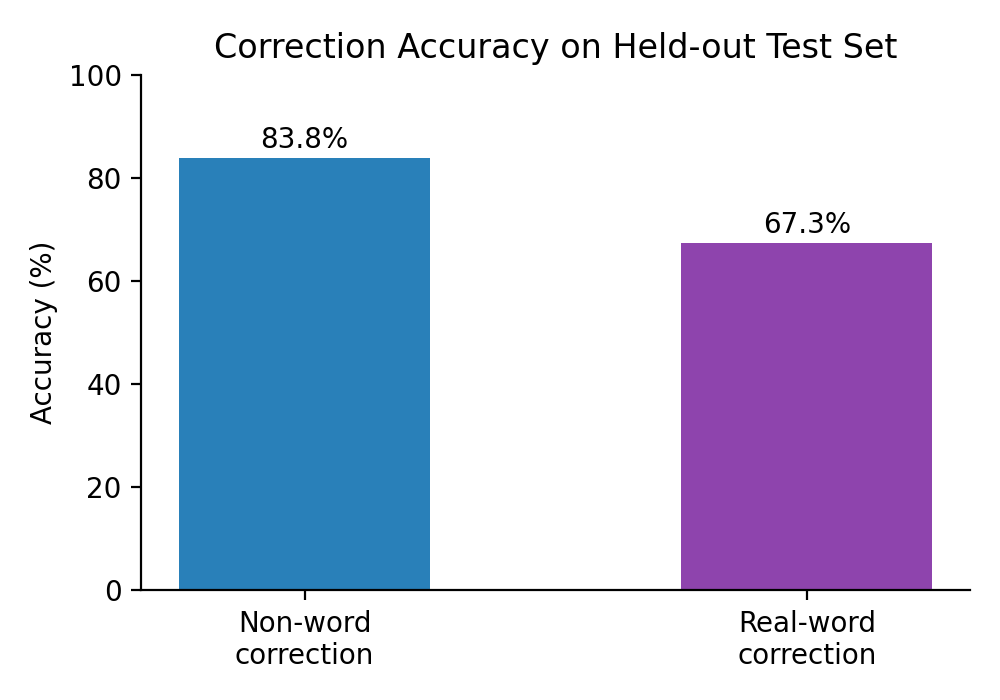
\includegraphics[width=0.7\textwidth]{assets/accuracy_chart.png}
\caption{Non-word vs. real-word correction accuracy.}
\label{fig:accuracy-chart}
\end{figure}

\begin{table}[H]
\centering
\begin{tabular}{lcc}
\toprule
\textbf{Method} & \textbf{Total time (1,000 words)} & \textbf{Speed-up} \\
\midrule
A --- Brute-force edit distance 1 & 0.1126~s & $1\times$ (baseline) \\
B --- Symmetric Delete & 0.0193~s & $\mathbf{5.8\times}$ \\
\bottomrule
\end{tabular}
\caption{Speed Demon benchmark results.}
\label{tab:speed-demon}
\end{table}

\paragraph{Why Method B wins.} Method A reconstructs the full set of edit-distance-1 strings \textit{from scratch} for every query, an $O(26n)$ operation dominated by the alphabet loop inside the \textit{replace} and \textit{insert} branches. Method B never performs an alphabet loop at query time at all: it only ever deletes characters from the query word ($O(n)$ deletions) and performs $O(n)$ hash lookups against a dictionary that was built once, offline, by pre-computing deletions of every vocabulary word. In other words, Method A pays the full combinatorial cost of relating a word to its neighbourhood on \textit{every query}; Method B pays a similar combinatorial cost only \textit{once}, during pre-processing, and reduces every subsequent query to cheap deletions and hash lookups. This is precisely the $\sim$5.8$\times$ speed-up observed empirically, and the gap would widen further for longer words or larger query batches, since Method A's per-query cost scales with $n$ while Method B's advantage compounds with reuse of the same pre-processed dictionary across queries.

\section{Part 5: Live Interactive Application}

The corrector is packaged as a continuous terminal CLI (\texttt{src/cli.py}): a \texttt{while True} loop reads one sentence at a time, corrects it via \texttt{correct\_sentence}, prints the corrected sentence with any changed words wrapped in \texttt{**asterisks**} (and, on ANSI-capable terminals, also rendered in bold green), and prints the wall-clock latency of the correction in milliseconds. The loop terminates when the user types \texttt{exit}.

\begin{figure}[H]
\centering
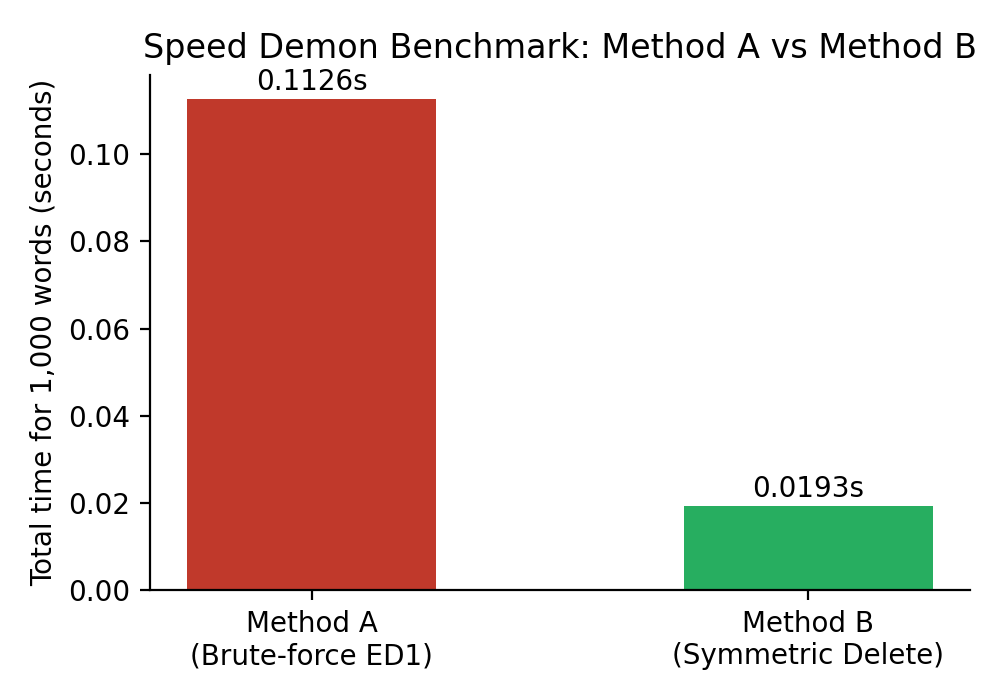
\includegraphics[width=0.7\textwidth]{assets/speed_demon_chart.png}
\caption{Total latency for 1,000 misspelled words, Method A vs. Method B.}
\label{fig:speed-demon-chart}
\end{figure}

\begin{lstlisting}[caption={Sample interactive session}, label={lst:session}]
================================================================
Spelling Corrector -- interactive mode
Type a sentence and press Enter. Type 'exit' to quit.
================================================================

> I hav a good feeling about this.
Corrected: I **had** a good feeling about this.
Changed:   hav -> had
Latency:   1.45 ms

> This is a test sentnce.
Corrected: This is a test **sentence**.
Changed:   sentnce -> sentence
Latency:   0.83 ms

> I would like to sea the world.
Corrected: I would like to **see** the world.
Changed:   sea -> see
Latency:   2.10 ms

> exit
Goodbye!
\end{lstlisting}

Note the third example: ``sea'' is a perfectly valid English word, so it is never flagged by vocabulary lookup alone; it is only corrected because the real-word pathway (Section~4) finds that ``I would like to see the world'' is significantly more probable under the bigram model than the original phrase.

\section{Discussion, Limitations, and Extensions}

\paragraph{Non-word vs. real-word accuracy gap.} The $\sim$17-point accuracy gap between non-word (83.8\%) and real-word (67.3\%) correction is consistent with the wider spelling-correction literature: context-dependent decisions are inherently harder than vocabulary-membership decisions, and a bigram model is a comparatively weak language model (it only ``sees'' one word of context on each side).

\paragraph{Smoothing choice.} Add-one (Laplace) smoothing was chosen for simplicity and interpretability; it is known to over-penalize frequent bigrams in favour of unseen ones on larger vocabularies. A production system would likely switch to a more sophisticated scheme (e.g. Kneser--Ney or Katz backoff) or a higher-order (trigram+) model, at the cost of additional implementation complexity.

\paragraph{The real-word margin $\tau$.} This single hyperparameter directly trades recall for precision on real-word correction: lowering $\tau$ would catch more genuine errors like ``meat'' $\rightarrow$ ``meet'' but would also risk more false-positive ``corrections'' of already-correct sentences. Tuning $\tau$ against a labeled validation set (rather than the fixed value used here) is a natural next step.

\paragraph{Scope.} Both candidate-generation methods are explicitly scoped to edit distance 1, per the assignment specification. Multi-error words (edit distance $\geq 2$) are out of scope and would require extending Method B's pre-processing to deeper deletion depths (which SymSpell natively supports) and Method A to a recursive edit-distance-2 generator.

\paragraph{Reproducibility.} All random sampling (test-set generation, Speed Demon batch construction) is seeded, so the numbers reported in Section~5 are exactly reproducible by re-running \texttt{python main.py evaluate}.

\section{Conclusion}

This assignment implements a complete, working spelling correction pipeline on top of the NLTK Brown corpus: a unigram/bigram language model (Part 1), two independent single-edit candidate generators with markedly different computational profiles (Part 2), frequency- and context-driven correction logic for non-word and real-word errors respectively (Part 3), an automated evaluation harness with an explicit head-to-head speed benchmark (Part 4), and a live, interactive terminal deployment (Part 5). The central empirical result --- Method B (Symmetric Delete) outperforming Method A (brute-force edit distance 1) by $\sim$5.8$\times$ on an identical workload --- is a direct, measurable consequence of moving the alphabet-sized combinatorial search from query time into a one-time pre-processing step, illustrating a classic and broadly applicable systems-design trade-off between pre-computation and per-query work.

\end{document}
